\documentclass{article}
% \usepackage[margin=1.5in]{geometry}
\usepackage[utf8]{inputenc}
\usepackage{enumitem}
\usepackage{titlesec}
\usepackage{minted}
\usepackage{listings}
\usepackage{parskip}
\usepackage{changepage}
\usepackage[backend=bibtex]{biblatex}
\usepackage{graphicx}
\usepackage{refcheck}
\usepackage[slovene]{babel}
\usepackage{wrapfig}
\usepackage{caption}
\usepackage{subcaption}
\usepackage{float}
\usepackage{csquotes}
\usepackage{mwe}

\graphicspath{ {./images/} }

\bibliography{refs}

% \title{Linux grafika od zahteve do prikaza}
% \author{Matic Poženel}
% \date{Julij 2024}

\begin{document}
\definecolor{bg}{rgb}{0.91,0.91,0.91}

\begin{titlepage}
    \begin{center}
        \vspace*{8em}

        \textbf{\Huge Linux grafika od zahteve do prikaza}

        \vspace{0.5em}

        Pregled grafičnega sklada v Linux operacijskih sistemih

        \vspace{5em}

        \textbf{\Large Matic Poženel}

        \vspace{3em}

        Predmet: Računalništvo v praksi

        Mentor: izr. prof. dr. Jurij Mihelič 

        \vspace{3em}

        Julij 2024

        \vfill
        \includegraphics[width=0.4\textwidth]{fri_logo}

        % Univerza v Ljubljani\\
        % Fakulteta za računalništvo in informatiko
        \vspace{3em}
    \end{center}
\end{titlepage}

\titlepage

\thispagestyle{empty}
\tableofcontents
\newpage
\thispagestyle{empty}
\listoffigures
\newpage
\pagenumbering{roman}

\begin{abstract}
    Pričujoče delo opisuje sestavo grafičnega sklada na operacijskem sistemu Linux.
    Opisuje posplošen model grafičnih skladov, nekaj osnov grafične strojne opreme --
    medpomnilnika okvirjev (angl. \textit{framebuffer device}), grafične procesne enote (GPE)
    in grafičnih kartic -- in pa posamezne komponente ter najpogostejše aplikacije,
    ki jih zasledimo na Linuxovih sistemih. To so (poleg jedra in gonilnikov) grafični API
    (OpenGL z implementacijo Mesa), podsistema DRM in infrastruktura DRI, okenski sistemi in
    prikazni strežniki (okenski sistem X in Wayland Compositor), kompozitor in ostala
    višjenivojska grafična orodja.

    Cilj je približati osnove grafičnega programiranja na Linuxu začetnikom na tem
    področju. Za razumevanje spodnjih konceptov je potrebno razumeti le nekaj osnov
    delovanja in organizacije računalniških sistemov ter delovanja Linux operacijskega sistema 
    (npr. sistemski klici). Navedeni primeri so napisani v jeziku C.

    Pričujoče delo \textbf{\textit{se ne poglablja}} v matematiko, ki opisuje računalniško 
    grafiko. Prav tako delo ni priročnik za uporabo katerekoli navedene knjižnice; tu ni opisov,
    katere funkcije in strukture sestavljajo OpenGL, okenski sistem X ali podsisteme Linux
    jedra, niti ni navodil za uporabo visokonivojskih orodij, kot je GTK+. Pričujoče delo
    zgolj daje izhodišče za začetnika, ta pa se lahko po svojih željah nato poglobi v
    posamezne dele grafičnega sklada.
\end{abstract}
\newpage
\pagenumbering{arabic}

\addcontentsline{toc}{section}{Uvod}
\section*{Uvod}
Po predmetu Vgrajeni sistemi sem postal precej navdušen nad programiranju mikroprocesorjev, predvsem zaradi enostavnosti programiranja. Pomnilniško preslikani naslovi omogočajo preprosto interakcijo z vhodno-izhodnimi napravami (V/I napravami) -- potrebno je poznati le specifikacijo in pomen bitov v njenih registrih.

Ob programiranju na višjem nivoju (native aplikacije z grafičnim vmesnikom) se mi je zato začelo porajati vprašanje -- zakaj je potrebno za vsak programski jezik mukotrpno iskati grafični vmesnik, ki bi zadovoljil potrebe programerja? Še več -- ali bi morda lahko spisal svoj grafični vmesnik, ki bi bil prilagojen mojim potrebam? Konec koncev je za delovanje računalnika zadolžen procesor in ta more na tak ali drugačen način sporočiti zaslonu, naj na koordinati (X,Y) aktivira piksel z neko določeno barvo.

\section{Grafični sklad}
Grafični sklad\autocite{osdev} je nabor programskih komponent, ki nadzirajo delovanje naprav (npr. gonilniki) in nudijo vmesnik za programiranje (API) z namenom prikaza grafičnih elementov na izhodni napravi.
Za grafični sklad sicer ni predpisane enotne oblike, a večinoma so plasti, ki ga sestavljajo, razporejene na sledeč način (nivo najbližje strojni opremi je na lestvici najnižje):

\begin{enumerate}
    \item Aplikacijska plast (Application layer)
    \item Interoperacijske plasti (Interoperation layer)
        \begin{enumerate}[label*=\arabic*.]
            \item Plast za nadzor namizja (Desktop Management Layer)
            \item Plast za nadzor oken (Window Management Layer)
        \end{enumerate}
    \item Predstavitvene plasti (Presentation Layers)
        \begin{enumerate}[label*=\arabic*.]
            \item Kompozicijska plast (Compositing Layer)
            \item Orodna plast (Widget Toolkit Layer)
            \item Upodobitvena plast (Rendering Layer)
        \end{enumerate}
    \item Prikazne plasti (Display Layers)
        \begin{enumerate}[label*=\arabic*.]
            \item Gonilniška plast (Device Driver Layer)
            \item Strojna plast (Hardware Layer)
        \end{enumerate}
\end{enumerate}

Omenimo še, da se tisti grafični skladovi, ki slonijo na okenskemu sistemu X nekoliko razlikujejo od ostalih, saj X uporablja ločena grafična skladova za strežnika in odjemalca zaradi svoje strežniške arhitekture \autocite{osdev}. To na primer pomeni, da aplikacijska plast praktično v celoti pripada odjemalcu, interoperacijske plasti pa strežniku.

V sledečih poglavjih bomo omenili tudi vmesnike, ki jih lahko uporabimo pri posameznih plasteh, kolikor je to mogoče, podrobneje pa jih bomo spoznali v poglavju, ki opisuje grafični sklad v operacijskih sistemih Linux.

\textbf{Opomba}: pri opisu funckionalnosti posameznih plasti je potrebno razumeti, da višje plasti večinoma predstavljajo le olajšavo našega dela\footnote{To se na primer razlikuje od plasti pri računalniških komunikacijah. Npr. transportna plast in omrežna plast imata dejansko različne namene in ju predstavljajo različni koncepti. Pri grafičnem skladu nam npr. upodobitvena plast le močno olajša delo -- vso kompleksno matematiko bi namreč lahko sprogramirali sami v zbirniku in delali neposredno v strojni plasti, a tak podvig bi bil neporedstavljivo zahteven.}. Obstajajo sicer plasti, ki prinesejo nove koncepte, kot je npr. plast za nadzor oken, a bi lahko kompleksno grafiko upodabljali tudi brez koncepta oken.

\subsection{Prikazna plast}
\subsubsection{Strojna plast}
V strojni plasti najdemo strojno opremo, torej fizične naprave, ki jih uporabljajo višje plasti.

Vmesnik za strojno plast je ponavadi kar pomnilniško preslikan vhod/izhod. Problem je, da moramo imeti dokumentacijo uporabljene strojne opreme, npr. grafičnih kartic, do katere pa se je zelo težko dokopati.

\subsubsection{Gonilniška plast}
Gonilniška plast vsebuje gonilnike, ki omogočajo delovanje bodisi specifičnih prikaznih naprav (video pomnilnika, GPE, zaslona ipd.), bodisi z neko pomnožico le-teh.

To ne pomeni, da vse sloni na gonilnikih -- standard VESA BIOS Extensions (VBE) definira vmesnik, ki ga programska oprema (v tem primeru je tu mišljen predvsem BIOS) lahko uporabi za dostop do medpomnilnika okvirjev grafične kartice.

Vmesnik za gonilniško plast v operacijskih sistemih Linux predstavlja kar jedro s sistemskimi klici \mintinline{C}{ioctl} oz. knjižnice, ki jih ovijajo, npr. \mintinline{C}{libdrm}, ter ogrodja, kot je DRI.

\subsection{Predstavitvene plasti}
\subsubsection{Upodobitvena plast}
Splošno pravilo upodobitvene plasti je, da se po nekem algoritmu iz navodil, matematičnih funkcij in podobnih abstraktnih konstruktov pridobi sliko (tj. neko grafično celoto), ki se bo izrisala na zaslon, in sicer prek posebnega programa -- upodobitelja (angl. \textit{renderer, rendering engine}) \autocite{renderer}. Tu nastane razkorak med 2D in 3D grafiko, saj se je potrebno, na primer, odločiti, s katerim principom se bodo izrisovala okna na zaslon. Čeprav se morda zdi, da bi lahko za vse probleme uporabljali le 3D upodabljanje (saj lahko na 2D gledamo kot na poseben primer 3D), je to računsko veliko bolj intenzivno in se na starejši strojni opremi ne obnese tako dobro, kot klasično 2D upodabljanje.

Vmesnik upodobitvene plasti predstavlja grafični API. Zelo prepoznavna je specifikacija OpenGL oz. knjižnica Mesa -- s tovrstnim orodjem povemo prikazni plasti (strojni in gonilniški plasti) naj za nas izračuna željene funkcije, ki nam vrnejo okvir.
Vlogo upodobitelja lahko igrajo naši programi, če neposredno izvajajo upodabljanje na GPE; tudi prikazni strežnik igra vlogo upodobitelja.

\subsubsection{Orodna plast}
Orodna plast večinoma skrbi za izris grafičnih kontrolnih elementov (gumbi, meniji, vnosna polja itd.), ki jih uporablja nadzornik oken. Ta plast je večinoma kar združena z upodobitveno plastjo. Grafični kontrolni elementi pa morajo (večinoma) delovati s kompozitorjem.

Vmesnik orodne plasti so GUI orodja, kot sta GTK+ in Qt -- ta v ozadju pogosto uporabljajo grafične API-je iz upodobitvene plasti. Ta plast je nemalokrat kar združena s kompozicijsko, saj morajo GUI pripomočki delovati s kompozitorjem.

\subsubsection{Kompozicijska plast}
V kompozicijski plasti se nahaja poseben program, imenovan kompozitor (kompozicijski upravljalec oken), ki skrbi za ustrezno razporeditev (kompozicijo) grafičnih elementov iz spodnjih plasti na zaslonu. Za 2D grafiko to plast nemalokrat kar enači z upodobitveno (z upodobitvene plasti), pri 3D grafiki pa je skoraj vedno samostojna.

Vmesnika za kompozicijsko plast ni preprosto določiti, saj je ta precej abstraktna, lahko pa izbiramo iz precej širokega nabora kompozitorjev, ko sestavljamo svoj grafični sklad.

\subsection{Medoperacijske plasti}
\textbf{Opomba}: Medoperacijske plasti in predstavitvene plasti so med seboj povezane in bi za nekatere posamezne plasti lahko rekli, da so na enakem nivoju -- primer sta npr. kompozicijska plast in plast za nadzor okenj.

\subsubsection{Plast za nadzor oken}
Grafično procesiranje in prikaz , kot sta bila razložena do te točke, se odvijata tako rekoč na enem platnu, poimenovanem "okno". Upravljalec oken jih lahko izriše več in določi, na katero bo pripadalo kateremu programu. Zadolžen je tudi za razporejanje oken, morebitno prekrivanje ipd.

Plast lahko enačimo s konceptom okenskega sistema. Obstaja več arhitektur: v nekaterih ga sestavljata prikaznega strežnika in upravitelja oken (npr. X), v drugih je edina komponenta kompozitor (npr. Wayland).

Tu se že srečamo z nekoliko bolj poznanimi (tržnimi) imeni, kot so AwesomeWM, qtile, i3wm in drugimi.

Vmesnik plasti za nadzor oken so knjižnice, s katerimi dostopamo do okenskega sistema -- npr. libwayland, Xlib, XCB in druge.

\subsubsection{Plast za nadzor namizja}
Upravljalec namizja je večinoma tista komponenta, na katero pomislimo, ko govorimo o grafičnih uporabniških vmesnikih (GUI-jih). Tudi tu srečamo poznana imena, kot so KDE, Gnome, XFCE, Cinnamon, MATE in drugi.

Vmesnik plasti za nadzor namizja je zopet abstrakten -- kot pri kompozicijski plasti lahko tudi tu izbiramo med številnimi namiznimi okolji, kot so navedena zgoraj (KDE itd.).

\subsection{Aplikacijska plast}
Aplikacijska plast je prepuščena programu, ki želi uporabljati računalniško grafiko. Včasih se lahko vloge te plasti pomešajo z vlogami nižjih plasti -- v okenskemu sistemu X se dandanes nemalokrat zgodi, da aplikacije že same poskrbijo za upodabljanje in grafične kontrolne elemente, nato pa samo sporočijo X strežniku, naj pridelane piksle izriše na okno.

Vmesnik aplikacijske plasti je zelo širok pojem, saj lahko glede na potrebe našega programa uporabimo vmesnik katerekoli plasti. Čeprav se lahko omejimo na prikazne plasti in z velikimi mukami programiramo v zbirniku, ponavadi raje uporabimo visokonivojske knjižnice, ki služijo kot ogrodje za grafični API. Primer take knjižnice je GLFW \autocite{glfw}.

\newpage

\section{Strojna oprema}
Brez vhodno/izhodnih (V/I) naprav nam računalniki bore malo koristijo. Če poenostavimo: želimo si imeti nek način vnosa podatkov v pomnilnik, ter nek način pridobivanja podatkov iz pomnilnika tako, da bodo človeku berljivi -- to pomeni, da želimo podatke pridobiti v grafični (besedilo, vizualizacije...), zvočni ali pa v kaki drugi, zaenkrat precej futuristični obliki. Ker se v pričujoči predstavitvi osredotočamo na grafično obliko, bomo izmed perifernih naprav zagotovo potrebovali zaslon. Sam način vhoda in izbira vhodnih perifernih naprav za potrebe te predstavitve ni bistvena (razen v določenih delih).
Vprašanje se torej glasi -- kako pripravimo procesor, da nam na zaslon izriše nekaj pikslov? Še bolje: kako to ukažemo Linux jedru \autocite{osdev}?

\subsection{Fizični medpomnilnik okvirjev (\textit{framebuffer device})}

\begin{wrapfigure}{O}{0.45\textwidth}
    \vspace*{10pt}
    \centering
    \includegraphics[width=0.8\linewidth]{Sun_sbus_cgsix_framebuffer2}
    \caption{Fizični medpomnilnik okvirjev \textit{Sun sbus cgsix}. \autocite{fig:sunbus}}
\end{wrapfigure}
\

Če preskočimo prikaze, osnovane na znakovnih celicah\footnote{Teh danes večinoma ni več, saj so nastali zaradi dragega spomina in dragih fizičnih medpomnilnikov okvirjev \autocite{textmode}. Danes gre vse prej ali slej skozi medpomnilnik okvirjev. Več o tem v nadaljevanju.}, so Linuxovi sistemi v začetku podpirali medpomnilnike okvirjev (MO, angl. \textit{framebuffer}). Sprva je bila to fizična naprava, ki je, kot je moč razbrati iz imena, hranila naslednji okvir (sliko oz. polje pikslov), ki se bo izrisal na zaslon v naslednji iteraciji. Poleg tega je nudila tudi vmesnik v obliki pomnilniško preslikanih registrov, prek katerega je bilo mogoče nastavljanje načina delovanja naprave oz. njen \mintinline{C}{mode} (ang. mode-setting). Tako kot sodobne grafične kartice je bil na napravi vgrajen vmesnik, na katerega je bil preko ustreznega kabla priključen zaslon. Za primer: medpomnilniku okvirjev je bilo mogoče prek pomnilniško preslikanih registrov sporočiti, da bo zaslon, ki je priključen na vmesnik MO, deloval z resolucijo $1920 \times 1080$ in frekvenco osveževanja $60$Hz.
To pomeni, da je bilo moč prek medpomnilnika okvirjev zaslon poganjati izven njegovih zmožnosti, kar je povzročilo fizično škodo na njem \autocite[Poglavje Display Modes]{framebuffer} \autocite{overdrive}.

\subsection{Grafične procesne enote}
Uporaba MO pa je bila poleg teh varnostnih hib precej neučinkovit pristop za upodabljanje 3D grafike. Upodabljanje, ki sloni skoraj izključno na linearni algebri (matričnih operacijah), je bilo še vedno prepuščeno procesorju. Tako so se začele pojavljati prve grafične procesne enote (GPE, angl. GPU).

Grafične procesne enote sestojijo iz enakih komponent, kot centralne procesne enote: oboje imajo aritmetično-logične enote, nadzorne enote in več nivojev predpomnilnikov. \autocite{framebuffer}

Razlikujeta pa se v številu in zmogljivosti posameznih komponent, in nenazadnje seveda v samem namenu. CPE je splošnonamenski -- s serijskim izvajanjem lahko stori vse, a morda nekoliko počasneje (npr. množenje matrik). GPE je namenjen predvsem za linearno algebro in paralelno računanje. Sestavljen je iz velikega števila jeder, ki računajo vzporedno druga z drugo. Hitrost grafičnih procesnih enot merimo v številu operacij v plavajoči vejici na sekundo (FLOPS, floating point operations per second), dandanes navadno v teraflopsih.

\begin{figure}[H]
    \centering
    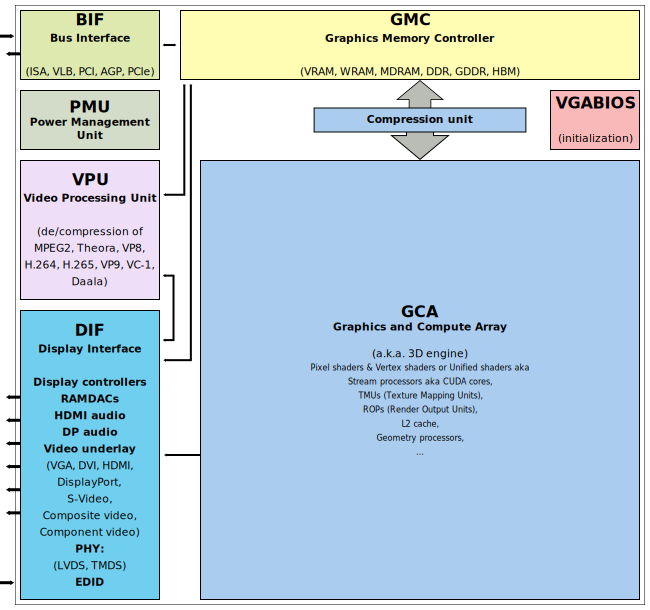
\includegraphics[width=0.75\linewidth]{Generic_block_diagram_of_a_GPU}
    \caption{Generična shema grafične procesne enote (GPU) \autocite{fig:genericgpu}.}
\end{figure}

\subsection{Grafične kartice}
GPE je lahko integriran (na istem vezju kot CPE), ali pa je na voljo kot samostojna naprava, ki ji pravimo grafična kartica. Integriran GPE si deli pomnilnik s CPE-jem, grafična kartica pa vsebuje svoj pomnilnik, imenovan video pomnilnik (VRAM), ki je namenjen izključno GPE in se po zasnovi nekoliko razlikuje od SDRAM-a (pogosto je to SGRAM oz. GDDR SDRAM, Graphics double data rate synchronous dynamic random-access memory). Na grafični kartici najdemo še vmesnik, na katerega lahko priključimo zaslon -- ta je bil doslej povezan bodisi z MO-jem ali pa matično ploščo.

GPE na VRAM-u shranjuje različne elemente grafičnega upodabljanja (npr. teksture) \autocite{cornell} in pa medpomnilnik okvirjev ter FIFO vrsta ukazov. MO pošilja okvirje na vmesnik za zaslon, uporabniške aplikacije pa izstavljajo ukaze na FIFO vrsto in konfigurirajo napravo.

Na tej točki v zgodovini je še vedno obstajal problem neposrednega dostopa do grafične strojne opreme s strani programov. Lahko se je zgodilo, da v MO piše več aplikacij naenkrat; enako velja za konfiguracijo naprave \autocite{sdram}. Nalogo reševanja tega problema nosi jedro operacijskega sistema.

\begin{figure}[H]
    \centering
    \includegraphics[width=0.75\linewidth]{Sapphire-Radeon-HD-5570-Video-Card}
    \caption{Grafična kartica Sapphire Radeon HD 5570 \autocite{fig:sapphireradeon}}
\end{figure}

\section{\textit{Primer}: uporaba virtualnega medpomnilnika okvirjev v Linuxu}
Ker je MO zastarel in ni več v uporabi, ga dandanes na sistemih Linux ne uporabljamo več na enak način (tj. vsaj ne z napravo \mintinline{C}{fbdev} \autocite{forbiddenprojects}) \autocite{ffmpeg}.

Kljub temu obstaja abstrakcija medpomnilnika okvirjev, oziroma kar virtualni\footnote{"Virtualni", ker programi ne razlikujejo, ali gre za bodisi fizični MO, bodisi za hrambo okvirjev nekje v pomnilniku računalnika, bodisi za hrambo okvirjev nekje v video pomnilniku (VRAM-u) grafične kartice.} medpomnilnik okvirjev (VMO), ki je še vedno uporabljen v današnjih Linux sistemih. Predstavlja MO neke grafične naprave (npr. GPE) \autocite{fbdevdocs}. S perspektive programerja gre za navadno datoteko oz napravo \mintinline{C}{/dev/fb*}, kjer znak \mintinline{C}{*} ponazarja številko VMO, če imamo poleg vgrajene strojen opreme še grafično kartico \autocite{fbdevdocs}. Tega lahko tudi kot programerji neposredno uporabimo. Poglejmo si primer na omenjenem operacijskem sistemu. Tukaj delo upodabljanja opravi CPE; z drugo besedo -- \mintinline{C}{/dev/fb0} ne podpira strojnega pospeševanja oziroma uporabe GPE \autocite{fbdevdocs}.
Predpogoj za uporabo \mintinline{C}{fb0} je, da se iz grafičnega vmesnika prestavimo v enega izmed teleprinterjev (teletypewriter)\footnote{Prevod pridobljen 13. 7. 2024 s portala PONS (sl.pons.com). Verjetno bi bil ustrezen prevod tudi "teletipkalnik".}. Namizno okolje (v mojem primeru se nahaja na \mintinline{C}{tty7}) namreč ne uporablja naprav \mintinline{C}{fb*} neposredno -- edini dostop do njih ima uporavljalec oken, zaradi česar sprememb ni mogoče videti.

Po opravljenem preklopu v na primer \mintinline{C}{tty2} lahko pričnemo z neposrednim pisanjem v medpomnilnik okvirjev. Privzeli bomo, da je to \mintinline{bash}{/dev/fb0}

Najpreprostejši primer uporablja le lupino; poženemo sledeči ukaz: \\

\centerline{\mintinline{bash}{cp /dev/random /dev/fb0}}

\mintinline{bash}{/dev/random} sproti generira naključne vrednosti, zato se bo ukaz prej ali slej zaključil z napako, da je na napravi zmanjaklo prostora (popisali smo celoten ekran).

Poizkusimo izrisati $2^{20}$ pikslov modro-zelene barve (RGB: $0, 255, 255$) v medpomnilnik okvirjev z uporabo sistemskega klica \mintinline{C}{write()}.
Prevedemo in poženemo naslednjo kodo: \autocite[predelana koda]{displaywithframebuffer}

\inputminted[linenos,breaklines,bgcolor=bg,fontsize=\small]{C}{simple_framebuffer.c}

Sedaj lahko poskusimo še nekoliko kompleksnejši primer, kjer izrišemo kvdarat. Preprosto prevedemo in poženemo naslednjo kodo: \autocite{displaywithframebuffer}

\inputminted[linenos,breaklines,bgcolor=bg,fontsize=\small]{C}{framebuffer_testing.c}

Strukturi \mintinline{C}{fb_fix_screeninfo} in \mintinline{C}{fb_var_screeninfo} \autocite{fbdevapi} nosita fiksne in spremenljive informacije o zaslonu. Fiksne morda niso tako zanimive s perspektive programiranja grafike (so pa morda zanimive s perspektive razvoja operacijskih sistemov\footnote{V fiksnih na primer najdemo polji \mintinline{C}{unsigned long mmio_start} in \mintinline{C}{__u32 mmio_len} -- prvo hrani začetek pomnilniško preslikanega V/I, slednje pa njegovo dolžino.}), razen polja \mintinline{C}{line_length}, ki nosi število pikslov v eni vrstici. Druga struktura je veliko bolj zanimiva:

\inputminted[linenos,bgcolor=bg,fontsize=\small]{C}{fb_var_screeninfo.h}

Telo funkcije \mintinline{C}{main()} torej pridobi fiksne in spremenljive podatke. Slednji vsebujejo tudi x in y resolucijo zaslona, odmik na x in na y ter število bitov na piskel. Iz tega lahko izračunamo velikost enega okvirja zaslona v bajtih in določimo pomnilniški naslov (v VMO!), kamor bomo v $i$-ti iteraciji postavili $i$-ti piksel. Seveda moramo prej VMO še preslikati v pomnilniški prostor CPE, kar storimo s sistemskim klicem \mintinline{C}{mmap}.
Sedaj lahko VMO tretiramo kot binarno datoteko -- podobno, kot bi tretirali BMP datoteko. V dvojni for zanki se pomikamo piksel za pikslom in vsakič spremenimo količino rdeče, zelene in modre barve (ter prosojnost). Na koncu le čakamo na vnos nekega znaka, da se nam program ne zapre prehitro.

Če si ogledamo še funkcijo \mintinline{C}{get_screeninfo()}, ki pridobi podatke, lahko opazimo, da to stori prek sistemskih klicev \mintinline{C}{ioctl()}. Ti bodo ponovno prišli v upoštev v poglavju DRM in DRI. Za argumente vzamejo datotečni deskriptor, strojno-odvisen ukaz in dodatne argumente (v tem primeru strukturo, kamor se zapišejo pridobljeni podatki.)

\section{Grafični sklad operacijskega sistema Linux}

Jedro Linux operacijskega sistema nima orodij, ki bi omogočala izris kompleksnih grafičnih elementov na zaslonu, kot so okna, animacije in podobno. To pomeni, da se implementacija grafike razlikuje od distribucije do distribucije. V mnogih, kot so Ubuntu, Mint, openSUSE in Fedora, je določena implementacija grafičnega sklada že vgrajena v samo distribucijo, v lažjih ("lightweight") distribucijah, kot sta Arch in Gentoo, pa mora uporabnik sam dodati gonilnike, upravljalca oken, kompozitor in druge gradnike.

\begin{figure}[H]
    \centering
    \includegraphics[width=0.9\linewidth]{glamor}
    \caption{Grafični sklad Linux operacijskega sistema z arhitekturo okenskega sistema Wayland, ki z uporabo XWayland emulira delovanje okenskega sistema X. \autocite{fig:graphicsstack}}
\end{figure}

Najpogostejše komponente (nekatere so neizogibne) operacijskega sistema Linux so: \autocite{baeldunggui}

\begin{enumerate}
    \item jedro in gonilniki naprav;
    \item grafični API (OpenGL in konkretna implementacija, npr. Mesa);
    \item upravljalec neposrednega upodabljanja (DRM) in infrastruktura neposrednega upodabljanja (DRI);
    \item okenski sistem (ponavadi X) \textit{ali pa} zgolj prikazni strežnik (arhitektura Wayland);
    \item kompozitor;
    \item Ostale komponente in orodja za razvoj (npr. \mintinline{C}{Qt})
\end{enumerate}

\subsection{Linux jedro in gonilniki naprav}

Ko govorimo o operacijskih sistemih Linux, najprej naletimo na jedro, saj je to najosnovnejši in najpomembnejši del vsake Linux distribucije in skrbi za delovanje računalnika nasploh.

Linux jedro vsebuje vse od gonilnikov (npr. grafičnih kartic), do podsistemov, ki uporabljajo te gonilnike in dostopajo do strojne opreme (kot je DRI -- infrastruktura za neposredno upodabljanje). Linux jedro (z vsebovanimi gonilniki) tako predstavlja gonilniško plast, ta pa skupaj s strojno plastjo (katero tvori strojna oprema) tvori prikazno plast.

Na Linuxovem grafičnem skladu obstaja veliko prepletanja med njegovimi plastmi, zato je dvema pomembnejšima deloma grafičnih gonilnikov -- grafičnemu API-ju in DRI-ju -- namenjeno posebno poglavje.

Grafični API je namreč po eni strani namenjen uporabniku in z njim delamo na višjem nivoju, po drugi strani pa mora že sam izdelovalec grafičnih kartic (npr. Nvidia) na nivoju elektrotehnike GPE zasnovati tako, da bo omogočal vse, kar zapoveduje standard.

Če želimo spisati svoj odprtokoden gonilnik s podporo OpenGL-a, kot je Nouveau za Nvidia grafične kartice, lahko uporabimo arhitekturo Gallium3D. Gre za množico vmesnikov in zbirko knjižnic, s katerimi lahko spišemo gonilnik na (večinoma) strojno-neodvisen način.
Projekt Nouveau je primer zbirke odprtokodnih gonilnikov za Nvidia grafične kartice izdelanih s pomočjo Gallium3D API-ja. To pomeni, da so vsi Nouveau gonilniki izdelani po OpenGL standardu. Nouveau je del projekta Mesa.

Poleg grafičnega API-ja, ki sega v upodobitveno plast, obstaja tudi infrastruktura neposrednega upodabljanja (DRI), ki je tesno povezana z okenskim sistemom X in tako povezuje gonilniško plast in interoperacijske plasti. O tem več v poglavju, namenjenemu infrastrukturi DRI in podsistemu DRM.

\subsection{Grafični API in OpenGL}
Grafični API je tisti del grafičnega sklada, ki nastopi takoj za prikazno plastjo. Namenjen je programerju, da ga uporabi za izrisovanje kompleksnejših grafičnih elementov na zaslonu (npr. trikotniki).

OpenGL (in njegova "nadgradnja" Vulkan), je standard oz. specifikacija \autocite{openglfaq} grafičnega API-ja. V prvi vrsti namenjen izdelovalcem grafičnih kartic, saj po teh navodilih izdelajo gonilnike za svojo opremo, za katero nato rečemo, da je kompatibilna z OpenGL standardom. Na tej točki še ne govorimo o (programski) implementaciji OpenGL-a -- ta se pojavi v obliki gonilnika grafičnega procesorja (oz. grafične kartice).

Če povzamemo: niti OpenGL-a niti Vulkana ne moremo opredeliti kot "knjižnjici", temveč kot "seznam navodil", katerim zadošča več gonilnikov in implementacij\footnote{Podobno, kot je v kontekstu podatkovnih baz SQL le specifikacija jezika, obstaja pa več implementacij} za odjemalca\footnote{Arhitektura okenskega sistema X (ki je najbolj pogost sistem na operacijskih sistemih Linux), tudi klient; Prevod pridobljen 13. 7. 2024 s portala PONS (sl.pons.com).}. 

\subsubsection{Mesa in grafični gonilniki}

Mesa (oz. Mesa3D) \autocite{mesadocs} je ena izmed bolj poznanih implementacij OpenGL (in Vulkan) standarda za odjemalca. Gre za dejansko grafično knjižnico, ki nastopa v obliki gonilnika. To pomeni, da projekt Mesa:

\begin{enumerate}
    \item nudi gonilnik za neko specifično grafično kartico (primer: že omenjeni Nouveau za Nvidia grafične kartice);
    \item nudi implementacijo knjižnice \mintinline{C}{libdrm}, ta pa nudi ovojne funkcije sistemskih klicev \mintinline{C}{ioctl}, s katerimi komuniciramo z grafično kartico. 
    \item nudi implementacijo specifikacije OpenGL, torej vse funkcije, ki jih predpostavlja specifikacija tega API-ja.
\end{enumerate}

\begin{wrapfigure}{o}{0.45\textwidth}
    \vspace*{10pt}
    \centering
    \includegraphics[width=0.8\linewidth]{Mesa}
    \caption{Shema odnosa implementacje Mesa (OpenGL API-ja) z nižjimi in višjimi nivoji. \autocite{baeldunggui}}
\end{wrapfigure}
\

Gonilnik grafične kartice je torej zadolžen za prevedbo visokonivojskih ukazov, ki so na voljo programerju, v strojno kodo, razumljivo grafičnemu procesorju. Do funkcionalnosti, ki jih omogočata grafična kartica in njen gonilnik, lahko dostopamo samo preko jedra, in sicer prek podsistema DRM, ki ga bomo spoznali v sledečem poglavju. Projekt Mesa nudi knjižnico \mintinline{C}{libdrm} -- ta je del podsistema Linux jedra, imenovanega DRM (Direct Rendering Manager, upravljalec neposrednega upodabljanja) \footnote{Glej poglavje \textit{DRM in DRI}}. Sam razvoj podsistema DRM iz zgodovinskih razlogov v okrilju projekta Mesa \autocite{drm}, kar je razlog za tako povezavo med jedrom in omenjeno knjižnico.

Kako pa deluje knjižnica, ki implementira specifikacijo OpenGL? Deklaracije funkcij, ki jih predpisuje API, so zapisane v zagavnih datotekah (npr. \mintinline{C}{gl.h}, \mintinline{C}{egl.h}, \mintinline{C}{eglext.h} itd.\footnote{Podrobnosti strukture knjižnice OpenGL ni predmet te naloge.}). Pri prevajanju naših programov moramo povezati ustrezno deljeno knjižnico (npr. za zaglavno datoteko \mintinline{C}{gl.h} moramo pri prevajanju z \mintinline{C}{gcc} uporabiti zastavico \mintinline{C}{-lGL}, da povežemo deljeno knjižnico \mintinline{C}{libgl.so}). S tem dejansko uporabimo implementacijo OpenGL.

V isto kategorijo kot Mesa spada tudi Direct3D, na katerega naletimo na Windows operacijskih sistemih. Omenimo še, da zaprtokodni gonilniki, ki jih proizvajalec za neko grafično kartico zamenjajo celotno hierarhijo od samega gonilnika do implementacije standarda.

\subsubsection{Povezava med upravljalci oken in OpenGL}
Standard OpenGL je namenjen upodabljanju 2D in 3D grafike in tako ne nudi funkcij za stvarjenje oken. Kljub temu predpostavlja, da na sistemu deluje nekakšen upravitelj oken -- v Linuxu je to povečini X. Zato moramo uporabiti še GLX podaljšek (GLX extension) okenskega sistema X, s katerim lahko posamezno OpenGL sceno vežemo na neko X okno in tako omogočimo X odjemalcem, da rišejo na vzpostavljena okna \autocite{glxwiki}. Na Windows sistemih lahko namesto GLX uporabimo vmesnik WGL.

Ker odvisnost od upravljalca oken oteži programiranje prenosljivih aplikacij, so avtorji standarda OpenGL zasnovali še vmesnik EGL, ki povezuje poljubnega upravljalca oken z upodobitvenim API-jem. EGL deluje tudi, če upravljalca oken ni.

\subsubsection{Cairo in Pixman}
Omenimo še knjižnico Cairo. Skrbi izključno za izrisovanje vektorske grafike, v grafičnem skladu pa spada podoben nivo kot Mesa implementacija. Cairo uporablja različna zaledja (angl. \textit{backends}), ki jih imenuje površine (angl. \textit{surfaces}). Mednje spadajo Xlib, OpenGL, slikovne datoteke in SVG datoteke \autocite{cairobackends}. Če površina podpira strojno pospeševanje, ga uporabi \autocite{cairo}. Če Cairo za svoje zaledje torej uporablja OpenGL ali Xlib je torej upodabljanje strojno pospešeno; upodabljanje direktno na sliko, pa ni \autocite{cairoimgsurfaces}. 

Pri izrisovanju na platna okenskega sistema X s knjižnico Xlib zaradi narave obeh knjižnic pri takem programiranju nastane veliko ponavljajoče se kode. Da bi rešili ta problem, je bila razvita deljena knjižnica Pixman, ki povezuje X in Cairo na nekoliko bolj uporabniku prijazen način. Med drugim Pixman nudi rasterizacijske algoritme in podporo za gradiente.

Cairo knjižnice večinoma ne uporabljamo neposredno, temveč prek orodij, kot je GTK+. Če je naš projekt enostavne narave, pa lahko za ozadje knjižnice uporabimo OpenGL.

\subsection{DRM in DRI}
Infrastruktura neposrednega upodabljanja (DRI, Direct Rendering Infrastructure) \autocite{dri} je ogrodje, ki uporabniški programski opremi brez privilegijev omogoča izstavljanje ukazov grafični strojni opremi brez konfliktov. Če nekoliko poenostavimo: DRI razreši problem hkratnega pisanja programov v medpomnilnik okvirjev tako, da vsakemu dovoli alokacijo dela video pomnilnika na nadzorovan način.

\begin{figure}[H]
    \centering
    \begin{subfigure}{.49\linewidth}
        \centering
        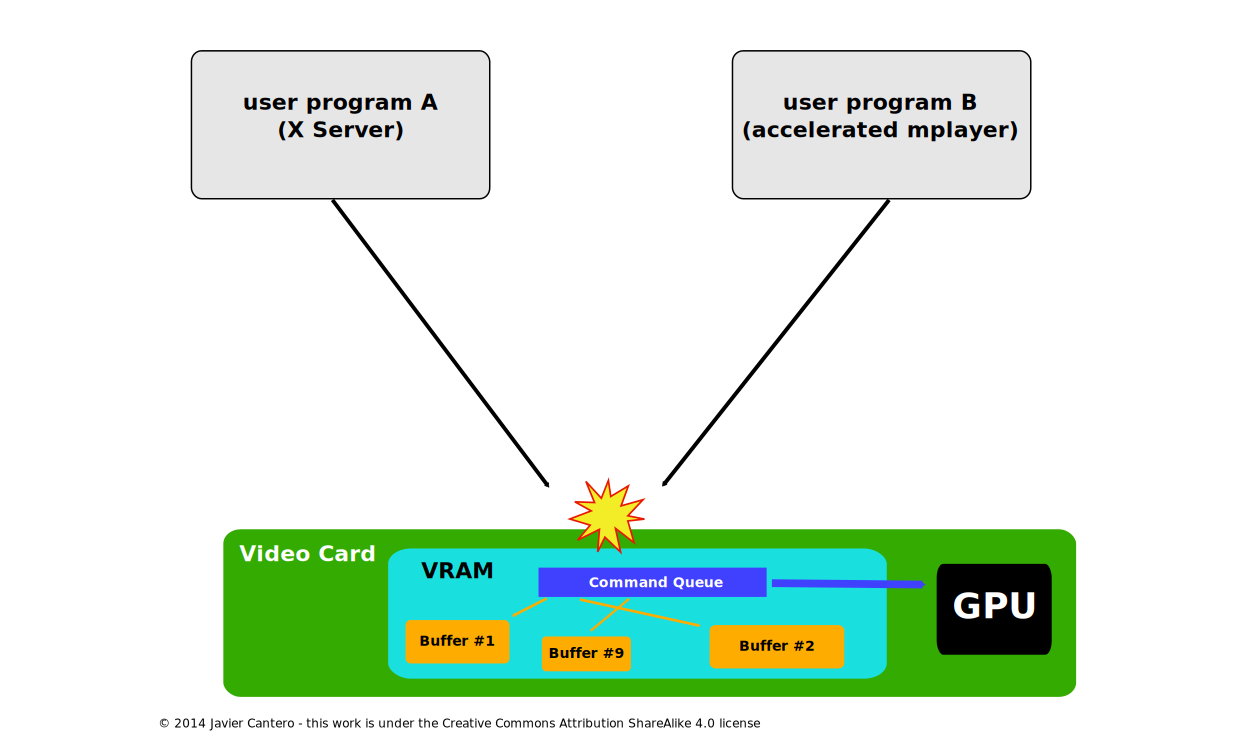
\includegraphics[height=100pt]{Access_to_video_card_without_DRM.png}
        \caption{Konflikti pri dostopanju večih programov do video pomnilnika. \autocite{fig:konflikti}}
    \end{subfigure}
    \begin{subfigure}{.49\linewidth}
        \centering
        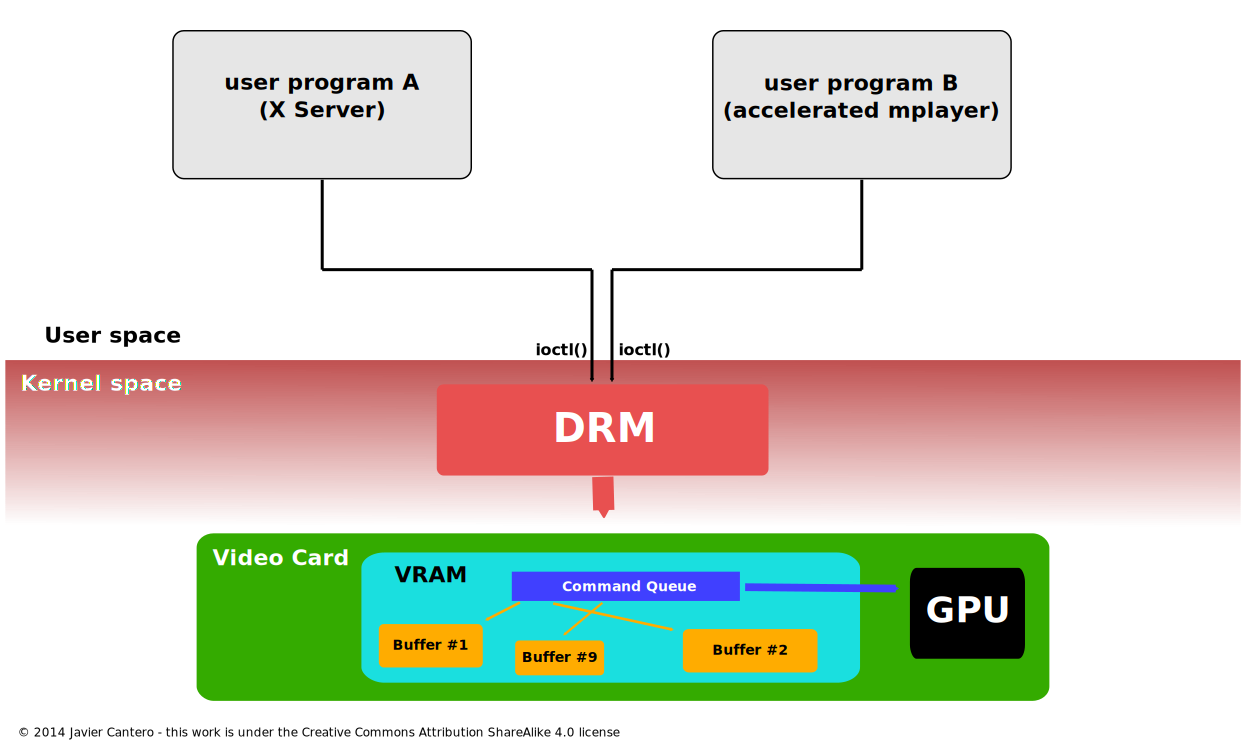
\includegraphics[height=100pt]{Access_to_video_card_with_DRM.png}
        \caption{Uporaba DRM odpravi problem hkratnega dotopa večih programov do video pomnilnika. \autocite{fig:nekonflikti}}
    \end{subfigure}
\end{figure}

Ime ogrodja izvira iz časov, ko je imel okenski sistem X edini pravico dostopanja do grafične strojne opreme (ta privilegij velja še danes), da bi se izognili konfliktom pri hkratnem dostopanju do nje. Tako so morali programi za izrisovanje najprej zahtevo predati X strežniku, od tod pa je bila zahteva posredovana grafični strojni opremi -- uporabljanje je bilo \textit{posredno}. Ob pojavu računsko-zahtevne 3D grafike je tovrstni model medprocesne komunikacije postal mnogo prepočasen. Iz tega razloga je bil razvit DRI, ki je omogočal \textit{neposredno} upodabljanje, tj. predajo ukazov grafični strojni opremi brez komunikacije z okenskim sistemom. Obstajajo tri različice DRI (DRI1, DRI2 in DRI3) -- sprva je vsak program pridobil edinstven nadzor nad grafično strojno opremo, z DRI2 pa jim je bila dana možnost alokacije video pomnilnika za upodabljanje. \autocite{dri}

Infrastruktura DRI je torej tesno povezana z okenskim sistemom X. Sestavljajo jo tri glavne komponente:

\begin{enumerate}
    \item \textbf{DRI odjemalec} je vsak program, ki od grafične strojne opreme zahteva storitve. Za delovanje potrebuje DRI gonilnike, ki navadno nastopajo v obliki deljenih knjižnic.
    \item \textbf{Okenski sistem X} nudi protokol X11, ki ga DRI odjemalci uporabijo za komunikacijo z okenskim sistemom -- z strojno-neodvisnim gonilnikom X -- in z strojno-odvisnim gonilnikom X. Slednji komunicira neposredno z grafično strojno opremo, zaradi česar se ga pogosto imenuje kar "video gonilnik" oz. "grafični gonilnik".
    \item \textbf{DRM (Upravljalec neposrednega upodabljanja)} je podsistem Linux jedra, ki nudi vmesnik GPE-jev in tako nadzira dostop do njih.
\end{enumerate}

\begin{figure}[H]
    \centering
    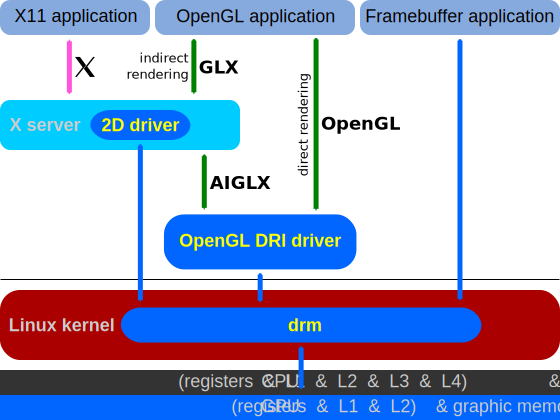
\includegraphics[width=0.75\linewidth]{Linux_graphics_drivers_DRI_current}
    \caption{Shema infrastrukture neposrednega upodabljanja. \autocite{fig:drischeme}}
\end{figure}

Morda je nekoliko manj očitno, da je vsak X odjemalec lahko tudi DRI odjemalec, saj lahko na primer zahteva upodabljanje od GPE, ta pa vrne upodobljen okvir\footnote{Okvir si lahko predstavljamo kot polje pikslov}. Temu postopku pravimo upodabljanje izven zaslona (off-screen rendering; GPE izvede upodabljanje, a ga ne izriše na zaslon).

Bolj očiten primer DRI odjemalca je X strežnik. Ta mora seveda uporabljati infrastrukturo, da lahko grafičnemu procesorju sporoči, kje se nahajajo posamezna okna. \autocite{dri}

Sedaj pa lahko razumemo učinkovitost infrastruktura neposrednega upodabljanja: X strežnik bo za vsak program, ki želi risati na zaslon, alociral kos video pomnilnika. Sedaj okvirja, ki je nastal pri upodabljanju zunaj zaslona, DRI odjemalcu ni potrebnopošiljati še X strežniku, da ga ta pošlje v video pomnilnik, temveč lahko programi povsem samostojno pišejo v svoj kos video pomnilnika, ta pa se izriše na zaslon -- tako se izognemo nepotrebni medprocesni komunikaciji. Če uporabnik spremeni velikost posameznega okna, bo X to preprosto sporočil ustreznemu odjemalcu in na novo alociral kos video pomnilnika. \autocite{dri}

Če kljub temu okvir najprej pošljemo X strežniku, pa lahko nad okvirjem izvedemo post-procesiranje.

\subsubsection{DRM}
Upravljalec neposrednega upodabljanja (DRM, Direct Rendering Manager) \autocite{drm} je podsistem Linux jedra, ki nudi vmesnik GPE-jev -- ti se v tem kontekstu imenujejo \textit{DRM naprave}. Vsako zaznano DRM napravo upravljalec razkrije programom v obliki datotek\footnote{princip ""\textit{Everything is a file}"} \mintinline{C}{/dev/dri/cardX}, kjer je $X$ zaporedna številka GPE. DRM uporablja sistemske klice \mintinline{C}{ioctl}, da alocira pomnilnik in nastavi parametre GPE. Sistemski klici \mintinline{C}{ioctl} so namenjeni za vhodno-izhodne operacije za različne naprave -- v tem primeru za GPE.

Definicija tega sistemskega klica je sledeča:\\

\centerline{\mintinline{C}{int ioctl(int fd, unsigned long request, ...)} \autocite{ioctldef}}

kjer so:

\begin{enumerate}[label=\arabic*.]
    \item \mintinline{C}{fd} odprt datotečni deskriptor naprave, ki jo naslavljamo;
    \item \mintinline{C}{request} ukaz, poslan napravi;
    \item \mintinline{C}{...} kazalec na nek kos pomnilnika, ki je iz zgodovinskih razlogov ponavadi \mintinline{C}{char *argp}.
\end{enumerate}

Da programerju ni potrebno "na pamet" poznati ukazov, ki jih lahko pošlje grafičnim karticam (sploh, ker se ukazi od ene do druge kartice razlikujejo), nam projekt Mesa nudi knjižnico \mintinline{C}{libdrm} \autocite[poglavje \textit{Software architecture}]{libdrm}, ki sestoji iz ovojnih funkcij posameznih ukazov za grafično kartico \autocite{drm}. Knjižnica ovija klice \mintinline{C}{ioctl} tako gonilnika Nouveau kot DRM \autocite{nouveauinstall}.

\begin{figure}[H]
    \centering
    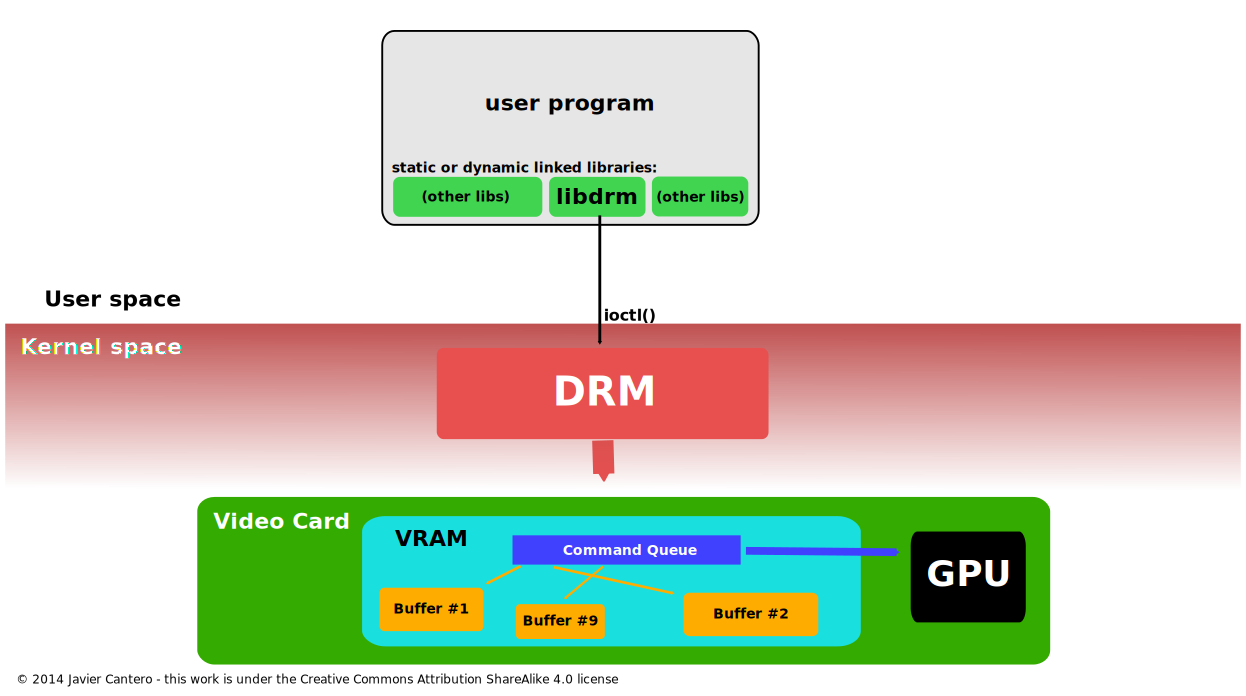
\includegraphics[width=0.75\linewidth]{High_level_Overview_of_DRM}
    \caption{Shema podsistema DRM. \autocite{fig:drmscheme}}
\end{figure}

DRM kot podsistem pa je sestavljen iz večih komponent; na kratko: \autocite{drm}

\begin{enumerate}
    \item \textbf{KMS (Kernel Mode Setting)} je komponenta, ki nam omogoča, da preko \mintinline{C}{libdrm} knjižnice neposredno konfiguriramo strojno opremo prek \mintinline{C}{ioctl} sistemskih klicev (angl. \textit{mode-setting}). KMS preprečuje, da bi programi sami neposredno nastavljali način delovanja grafične strojne opreme -- dandanes je X strežnik edini, ki ima pravice za uporabo KMS (seveda ob predpostavki, da sistem uporablja X sistem oken).
    \item \textbf{GEM (Graphics Execution Manager)} je komponenta, ki programom nudi API za upravljanje z video pomnilnikom. Možno je ustvariti, rokovati in uničiti ti. GEM objekte (ti predstavljajo podatke, ki jih potrebuje GPU -- npr. teksture). Programi si lahko isti GEM objekt med seboj delijo.
    \item \textbf{Upodobitvena vozlišča (Render nodes)} so posledica arhitekture pravic podsistema DRM. Ker v priviligiranem načinu delujejo le programi, ki nadzirajo izris (X strežnik, Wayland kompozitor...), mora vsak nepriviligiran program za uporabo GPE (pa čeprav ni v grafične namene) zaprositi priviligirani program. Upodobitveno vozlišče poleg datoteke \mintinline{C}{/dev/dri/cardX} nudi še datoteko \mintinline{C}{/dev/dri/renderDY} (številki $X$ in $Y$ nista nujno enaki\footnote{Na sistemu avtorja obstajata \mintinline{C}{/dev/dri/card0} in \mintinline{C}{/dev/dri/renderD128}.}), preko katere lahko vsak nepriviligiran program z nekoliko omejenim naborom ukazov prek sistema DRM izvaja računske operacije na GPE.
\end{enumerate}

\subsection{\textit{Primer}: uporaba DRM, KMS, GBM in OpenGL za strojno-pospešen grafični prikaz}
Z uporabo podsistema DRM in njegovih komponent KMS ter GBM (del projekta 
\begin{wrapfigure}{o}{0.25\textwidth}
    \centering
    \includegraphics[width=0.25\textwidth]{kmscube-image}
    \caption{Upodobitev aplikacije \mintinline{Bash}{kmscube}. Lastno delo.}
\end{wrapfigure}
Mesa) je moč izrisovati na zaslon s strojnim pospeševanjem. Poleg tega lahko uporabimo še funkcionalnosti, ki jih ponuja OpenGL in tako zagotovimo nekoliko zanimivejši rezultat.

Primer takega programa je na voljo na repozitoriju projekta Mesa in nosi naslov \mintinline{C}{kmscube} (gitlab.freedesktop.org/mesa/kmscube)\autocite{kmscube}. Zagon tega programa je enak kot v prejšnjem primeru -- prestavimo se v teleprinter \mintinline{C}{tty*}, prevedemo projekt z uporabo orodij Meson in Ninja, ter poženemo prevedeno datoteko. Program je precej kompleksen zaradi svoje nizkonivojske narave, zaradi česar se vanj ne bomo spuščali. Omenimo pa nekaj osnovnih lastnosti programa:

\begin{enumerate}
    \item Program uporablja knjižnico EGL \autocite{egl}, ki omogoča, da OpenGL uporabimo brez upravljalca oken, torej z neposrednim nadzorom nad medpomnilnikom okvirjev.
    \item S podsistemom KMS nastavimo delovanje grafične kartice.
    \item S podsistemom GBM \autocite{wikimesa}, ki je abstrakcija funkcij za upravljanje s pomnilnikom grafične kartice, alociramo medpomnilnik za grafično upodabljanje.
    \item OpenGL funkcionalnosti se kažejo predvsem v kompleksnem objektu, ki ga izrišemo -- 3D kocka.
\end{enumerate}

\subsection{Okenski sistemi}
Okenski sistem je del programske opreme, ki služi kot temelj grafičnega uporabniškega vmesnika tako, da realizira paradigmo WIMP \autocite{wikiwindowingsystem, stackwindowingsystem} -- okna, ikone, meniji, kazalci (\textbf{w}indows, \textbf{i}cons, \textbf{m}enus, \textbf{p}ointer). Gre za t.i. grafične nadzorne elemente (angl. \textit{graphical control element}) oz. grafične pripomočke (angl. \textit{graphical widget}).

Okenski sistem je sestavljen iz dveh delov, ki pa nista nujno ločena:

\begin{enumerate}
    \item \textbf{Prikazni strežnik} je osrednji del okenskega sistema. Vsak program z GUI-jem je njegov odjemalec. Njegova glavna naloga je nadzor vhodnih in izhodnih podatkov za odjemalce -- od njih pridobi zahteve za risanje na zaslon, pošilja pa jim uporabnikove kretnje (podatki s tipkovnice, miške, mikrofona itd.). Prikazni strežnik je tisti, ki komunicira s strojno opremo preko jedra. \autocite[poglavje \textit{Display server}]{wikiwindowingsystem}
    \item \textbf{Upravljalec oken} nadzira postavitev in izgled oken na zaslonu. Ne komunicira s strojno opremo, temveč le izdaja navodila za izris prikaznemu strežniku. \autocite{wikiwindowmanager}. V X arhitekturi je upravljalec oken le še en odjemalec prikaznega strežnika \autocite{howxworks}. 
\end{enumerate} 

\subsubsection{Upravljalec oken}
Poznamo več vrst upravljalcev oken: \autocite{wikiwindowmanager}

\begin{enumerate}
    \item \textbf{Skladovni upravljalci oken} omogočajo lebdeča okna, ki se lahko prekrivajo. Poznamo različne algoritme (slikarski algoritem, obratni slikarski algoritem) za izrisovanje teh oken.
    \item \textbf{Ploščični upravljalci oken} okna razporedijo v nekakšno polje, enega ob drugega. Tako ne pride do prekrivanaja.
    \item \textbf{Dinamični upravljalci oken} lahko dinamično preklapljajo med skladovnim in ploščičnim načinom razporejanja oken.
    \item \textbf{Kompozicijski upravljalci oken}, znani tudi kot \textbf{kompozitorji}, izrišejo vsa okna v izven-zaslonski pomnilnik (angl. \textit{off-screen buffer}). To omogoča post-procesiranje in dodajanje raznih 3D efektov in animacij. \autocite{wikicompositingmanager}
    \item \textbf{Namizna okolja} so posebna kategorija, saj poleg upravljalca oken nudijo še več orodij, kot so razne teme (angl. \textit{themes}), GUI brskalniki datotek in podobno.
\end{enumerate}

\textit{Namig}: da ugotovimo, katerega upravljalca okenj uporablja naš sistem, lahko zaženemo ukaz \mintinline{Bash}{rmctrl -m}.

\subsubsection{Okenski sistem X}
Okenski sistem X (na kratko: X) je odprtokoden okenski sistem, najdemo pa ga na večini današnjih linux sistemov. Organiziran je v zvezo odjemalec-strežnik in tako omogoča tudi oddaljen dostop.
X je eden izmed najbolj osnovnih gradnikov grafičnih uporabniških vmesnikov, zadolžen pa je tudi za rokovanje z dogodki (event handling) in za olepšave (visual decorations). \autocite{wikixsystem, howxworks}

X ima za prikazni strežnik omišljeno svojo rešitev: X.org. Strežnik navadno zažene upravljalec prikaza (angl. \textit{display manager})\footnote{Upravljalec prikaza je program, ki omogoča izbiro med različnimi okenskimi sistemi ter nemalokrat nudi tudi prijavno okno.} ali pa ga ročno zaženemo prek ukaznega poziva. \autocite{baeldunggui, wikixorg}

\begin{figure}[H]
    \centering
    \includegraphics[width=\linewidth]{Linux_Graphics_Stack_2013}
    \caption{Celoten grafični sklad v Linux operacijskem sistemu z okenskim sistemom X}
\end{figure}

Za komunikacijo med X strežnikom in X odjemalci se uporablja protokol X11 \autocite{baeldunggui, wikixorg}. Ta definira izmenjavo sporočil v strežniški arhitekturi sistema X. Če se strežnik in odjemalec nahajata na isti napravi, se sporočila izmenjajo z UNIX vtiči.
X11 je razširljiv -- nove funkcionalnosti lahko dodajamo brez spreminjanja protokola samega.

\mintinline{C}{Xlib} (X library) je knjižnica, namenjena implementaciji na strani odjemalca. Uporabljajo jo druga orodja, kot sta GTK+ in Qt za izdelavo grafičnih vmesnikov za aplikacije.

X.org Foundation dandanes odsvetuje razvoj aplikacij z neposredno uporabo X knjižnic, temveč priporoča različna orodja (dve omenjeni zgoraj). Za nizko-nivojski razvoj prav tako odsvetujejo uporabo \mintinline{C}{Xlib} knjižnice \autocite{xorgdocs}, priporočajo pa njeno "novejšo verzijo" oz. alternativo \mintinline{C}{XCB} (X C Binding). Razlogi so manjša velikost, večja odpornost na napake programerja, boljša podpora za multithreading, več razširitev in nižje latence \autocite{xcb}.

\subsubsection{Wayland}
Okenski sistem X je že precej star (prva verzija je zaživela leta 1984) in posledično postaja neroden za uporabo, predvsem zaradi pojavitve novih konceptov, kot so kompozitorji -- v arhitekturi sistema X se strežnik sploh ne zaveda lokacije oken na zaslonu in drugih specifik. Odjemalci morajo torej za izrisovanje zahtevo najprej poslati prikaznemu strežniku, ta jo odpošlje kompozitorju, od tod gre obdelana nazaj v strežnik in naposled do strojne opreme. Celoten proces se ponovi v obratnem vrstnem redu, ko uporabnik pritisne na nek grafični pripomoček, kot je gumb. 

Poleg tega dandanes porvprečen uporabnik ne potrebuje arhitekture z okenskim strežnikom, na katerega bi se povezalo več naprav, ki potrebujejo uporabljanje; ta zasnova pa zapovrh ni varna, saj ne kriptira oz. ne ščiti komunikacij med odjemalcem in strežnikom, kar omogoča prisluškovanje in potencialno razkritje zaupnih informacij.

\begin{figure}[H]
    \centering
    \begin{subfigure}{.49\textwidth}
        \centering
        \includegraphics[height=150pt]{x-architecture}
    \end{subfigure}
    \begin{subfigure}{.49\textwidth}
        \centering
        \includegraphics[height=150pt]{wayland-architecture}
    \end{subfigure}
    \caption{Primerjava X arhitekture (levo) in Wayland arhitekture (desno). \autocite{fig:waylandcomparison}}
\end{figure}

Wayland je naslednik okenskega sistema X. Nadomešča tako protokol X11 s protokolom Wayland, kot arhitekturo. Namesto strežnika postavlja kar kompozitor (ta mora biti kompatibilen z Wayland sistemom), s čimer se izogne nepotrebni medprocesni komunikaciji. Zahteve odjemalcev gredo zdaj zgolj čez kompozitor.

Pomemben gradnik Wayland arhitekture je knjižnica za medprocesno komunikacijo libwayland, ki kodira in dekodira sporočila ter jih pretvarja XML definicije sporočil v API, spisan v jeziku C \autocite{wayland}.

\begin{figure}[H]
    \centering
    \includegraphics[width=0.75\linewidth]{Wayland_display_server_protocol}
    \caption{Celoten grafični sklad v Linux operacijskem sistemu z Wayland arhitekturo \autocite{fig:wayland}}
\end{figure}

Kot je že moč razbrati, Wayland ponuja preprosto nadaljno vzdrževanje, razvijanje in razširjevanje.Kljub teoretično odlični arhitekturi je Wayland v času pisanja tega dela v povojih in zaradi številnih pomanjkljivosti, hroščev in napak povzroča številne preglavice, zaradi česar je X še vedno bolj popularna opcija.

Zaradi lažje kompatibilnosti v času, ko še vedno prevlada prikazni strežnik X, lahko uporabimo orodje XWayland, ki pod implementacijo Wayland arhitekture vrine še X strežnik in tako omogoči, da novejši protokol uporabijo tudi aplikacije, ki niso namenjene zanj.

\subsection{GUI orodja}
GUI orodje (tudi GUI knjižnica) vsebuje vse potrebne funkcionalnosti za izdelavo grafičnih uporabniških vmesnikov (GUI -- Graphical User Interface), kot so rokovalniki dogodkov, prizori (scene) in grafični pripomočki (angl. \textit{widgets}) \footnote{Prevod pridobljen 13. 7. 2024 s portala PONS (sl.pons.com). Beseda \textit{widget} izvira iz besede \textit{gadget}, \autocite[Glej poglavje History]{wikiwidget} kar v prevodu pomeni pripomoček. Glede na to, da nam "\textit{widget}-i" pomagajo pri interakciji z grafičnim vmesnimkom, jih lahko smatramo kot pripomoček in je posledično prevod razumen.}. 

Vsi sestavni elementi paradigme WIMP \autocite{wikiwindowingsystem, stackwindowingsystem} (okna, ikone, meniji, kazalci -- \textbf{w}indows, \textbf{i}cons, \textbf{m}enus, \textbf{p}ointer) predstavljajo grafične pripomočke, ki služijo interakciji med uporabnikom in računalnikom; uporabnik s klikom na gumbe, premiki oken in izbiranjem v menijih sporoči okenskemu sistemu, da želi določenemu programu poslati določene informacije, ki jih s svojim grafičnim vmesnikom definira program. Če npr. kliknemo na pripomoček za zapiranje oken, bo okenski sistem o tem obvestil ustreznega odjemalca, ta pa se bo na dogodek odzval.

V večini primerov so GUI orodja le ovojne knjižnice nizkonivojskih knjižnic, kot sta Xlib in XCB. Nekateri imajo celo implementirane lastne označevalne jezike, sisteme za dogodke in končne avtomate. Poglejmo si dve izmed bolj popularnih GUI orodij

\begin{figure}[H]
    \centering
    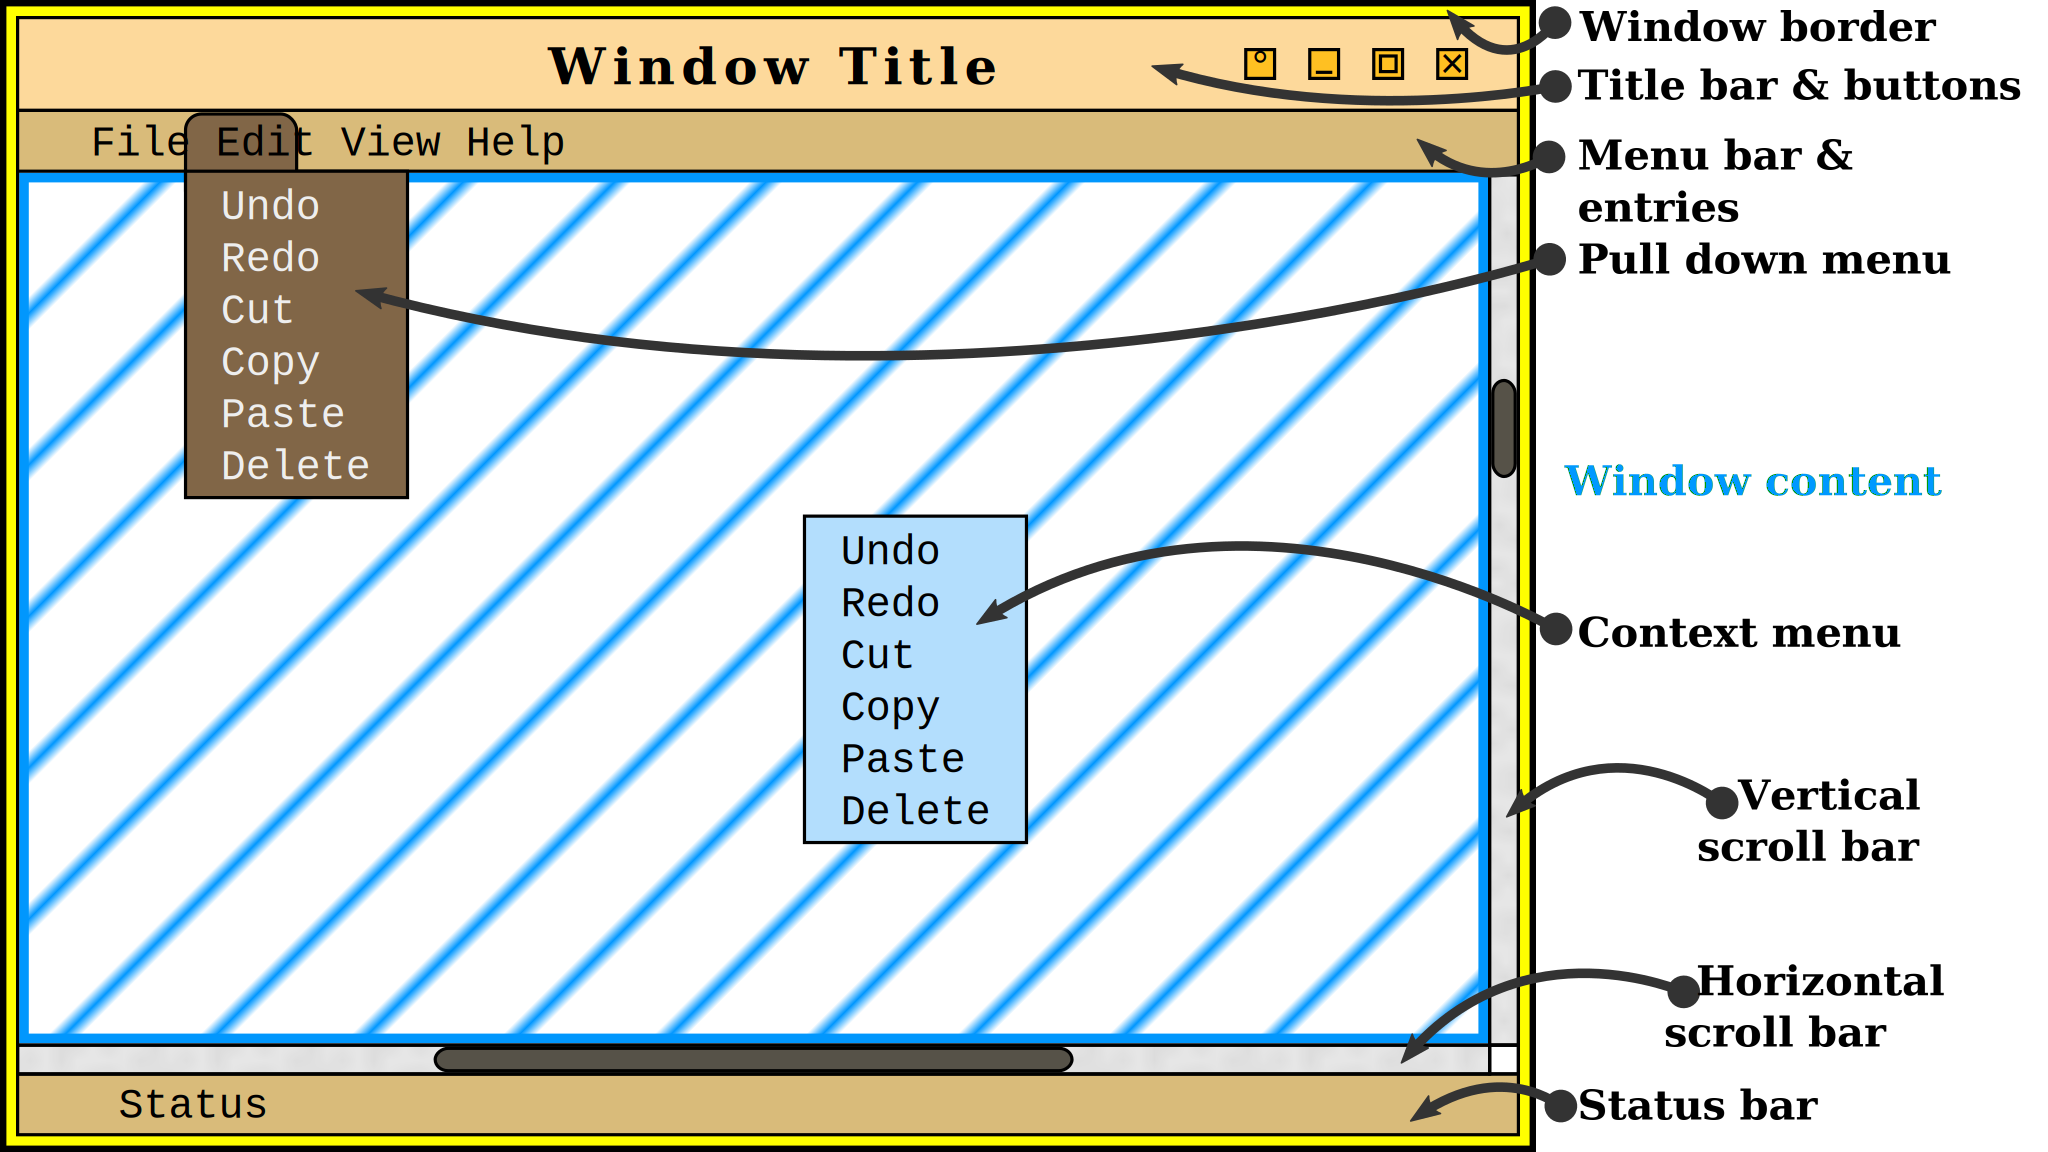
\includegraphics[width=\linewidth]{Winwow_windowing_system}
    \caption{Poglavitni deli okna (meniji), ki so tudi sami grafični pripomočki. \autocite{fig:windowsystem}}
\end{figure}

\newpage

\begin{wrapfigure}[5]{O}{0.6\textwidth}
    \vspace*{10pt}
    \centering
    \includegraphics[width=0.8\linewidth]{filechooser}
    \caption{Primer GUI-ja, zgrajenega z orodjem GTK+. \autocite{fig:filechooser}}
\end{wrapfigure}
\
\subsubsection{GTK+}
GIMP Toolkit je GUI orodje za izdelavo večplatformskih aplikacij z uporabniškim grafičnim vmesnikom.

\vspace*{8em}

\begin{wrapfigure}[12]{I}{0.6\textwidth}
    \vspace*{10pt}
    \centering
    \includegraphics[width=0.8\linewidth]{windows-style2}
    \caption{Primer GUI-ja, zgrajenega z orodjem Qt. \autocite{fig:calendar}}
\end{wrapfigure}
\
\subsubsection{Qt}
Qt je GUI orodje za izdelavo večplatformskih aplikacij z uporabniškim vmesnikom, ki ponuja knjižnico interaktivnih elementov, za razliko od GTK+ orodja pa lahko za izdelavo vmesnikov uporabimo aplikacijo QtDesigner in integrirano razvojno okolje (IDE) QtCreator.

\subsection{Ostali grafični vmesniki}
Čeprav je na tej točki že razvidno, da na Linuxu ne obstaja namensko orodje ali knjižnica za izdelavo uporabniških grafičnih vmesnikov, lahko opazimo, da (prej ali slej) vsi grafični ukazi v Linuxovem grafičnem skladu uporabijo OpenGL. To pomeni, ga da lahko kot Linuxovo namensko orodje za grafiko. Primer programa, ki deluje na opisan način, je Blender, ki se ne zanaša na nizkonivojske knjižnice ali orodja, temveč ima svojo knjižnico, popolnoma osnovano na standardu OpenGL \autocite{blendergui}.

Razvijalec lahko na višjem nivoju uporabi tudi knjižnice, ki so prenosljive med operacijskimi sistemi in prijazne za uporabo. Prier take knjižnice je GLFW (angl. \textit{Graphics Library Framework}). Je majhna knjižnica za uporabo OpenGL API-ja ter omogoča stvarjenje oken in celo rokovanje z vhodom (npr. miška, tipkovnica in igralna palica) \autocite{glfwwiki, glfw}.

\newpage

\addcontentsline{toc}{section}{Zaključek}
\section*{Zaključek}
Računalniška grafika ni enostavno področje. Odrkili smo le površino tega, kar je zmožno z današnjo grafično strojno opremo in koncepti, ki jih za sabo prinese samo upodabljanje.

Kljub temu lahko odgovorimo na nekaj vprašanj, ki se lahko porodijo začetniku.

\begin{enumerate}
    \item \textbf{Kako izrisati piksel na zaslon?} Uporabimo medpomnilnik okvirjev, ki se danes večinoma nahaja na grafični kartici. Do njega dostopamo prek mehanizmov Linux jedra, kot je \mintinline{Bash}{/dev/fb0}. To ni strojno-pospešen pristop, saj za upodabljanje uporabljamo procesor.
    \item \textbf{Kako izrisati piksel na zaslon z grafičnim pospeševanjem?} Na Linux sistemih bo potrebno uporabiti OpenGL (ali drug API), DRM in DRI.
    \item \textbf{Zakaj je treba za vsak programski jezik mukotrpno iskati grafični vmesnik?} V resnici ni potrebno; za prenosljivo aplikacijo bo dovolj uporabiti Qt ali pa GTK+.
    \item \textbf{Kako naj moj C ali Rust program (ali pa program v kateremkoli jeziku) sporoči računalniku, da želi nekaj narisati na zaslon?} Potrebno je vedeti, kateri okenski sistem uporablja naš računalnik. Nato ga z ustreznimi knjižnicami, ki pridejo z okenskim sistemom, zaprosimo za okno, na katerega lahko nato rišemo. To je prvi korak pri programiranju na računalniku z okenskim sistemom.
    \item \textbf{Kako sprogramiram svojo GUI knjižnico?} Za tak podvig bo skoraj vedno potrebno uporabiti OpenGL (ali drug API). Glede na to, katero plast bo predstavljala taka knjižnica, bo potrebno uporabiti bodisi knjižnico okenskega sistema, bodisi sistemske klice ipd.
\end{enumerate}

\addcontentsline{toc}{subsection}{Kam naprej?}
\subsection*{Kam naprej?}
Vsak, ki želi razumeti matematične postopke upodabljanja, programiranje lastnega upodobitelja ipd. lahko razišče področje \textbf{grafičnega cevovoda (angl. \textit{graphics pipeline})}.

Za ne-grafično programiranje GPE sta na voljo ogrodje CUDA podjetja Nvidia (za GPE-je tega podjetja) ali pa OpenCL (za splošno, odprtokodno ogrodje).

\newpage
\printbibliography

\end{document}
